% Brilliant documentation:
% http://mirror.ox.ac.uk/sites/ctan.org/macros/latex/contrib/beamer/doc/beameruserguide.pdf

\usepackage{beamerthemesplit}
\usepackage{textpos} 
\usepackage{hyperref}
\usepackage{graphicx}
\usepackage{calc}
\newlength{\popupimagewidth}

\setlength{\popupimagewidth}{\textwidth*3/5}

\addtobeamertemplate{frametitle}{}{
  % From http://tex.stackexchange.com/a/180628
  \begin{textblock*}{100mm}(\textwidth,-1cm)
    
\includegraphics[height=1cm,width=1cm]{ise-logo.jpg}
  \end{textblock*}
}

\title{Linked Open Data in Action}
\author{Matt Wallis}
\date{\today}

\begin{document}

\frame{\titlepage}

\section[Outline]{}
\frame{\tableofcontents}

\section{Introduction}
\frame
{
  \frametitle{Institute for Solidarity Economics}
  \begin{center}
    
\includegraphics[height=2cm,width=2cm]{ise-logo.jpg}
  \end{center}
  \begin{itemize}
    \item<1-> What is Solidarity Economics (very very very briefly)?
    \item<2-> \url{http://solidarityeconomics.org}
  \end{itemize}
}
\subsection{Philosophy}
Here's something between frames that appears only in the article.
\frame
{
  \frametitle{Principles}
  \begin{itemize}
    \item Receptive
    \item Open
    \item Value other people
    \item Empathy
    \item Walk a mile in someone else's shoes
    \item No room for ego
  \end{itemize}
}
\frame
{
  \frametitle{Principles applied to Software Engineering}
  \begin{itemize}
    \item Research what's already out there
    \item Re-use existing work
    \item Publish openly
  \end{itemize}
}
Our work is available on GitHub: \url{https://github.com/p6data-coop/ise-linked-open-data}
\section{Data}
\frame
{
  \frametitle{Why data?}
  \begin{itemize}
    \item
  \end{itemize}
}
\subsection{Linked Open Data}
\frame
{
  \frametitle{Overview}
  \begin{itemize}
    \item
  \end{itemize}
}
\frame
{
  \frametitle{ESSGLOBAL}
  \begin{itemize}
    \item
  \end{itemize}
}
\section{Applications}
\subsection{Example map application}
\frame
{
  \frametitle{map-app}
  \begin{itemize}
    \item Web application: \url{http://data.solidarityeconomics.org/map-app/}
    \item Data is loaded by querying our Linked Open Database (aka a Triple Store)
    \item Clean separation of application and data
  \end{itemize}
}
\frame
{
  \frametitle{Links in practice}
  \begin{center}
    %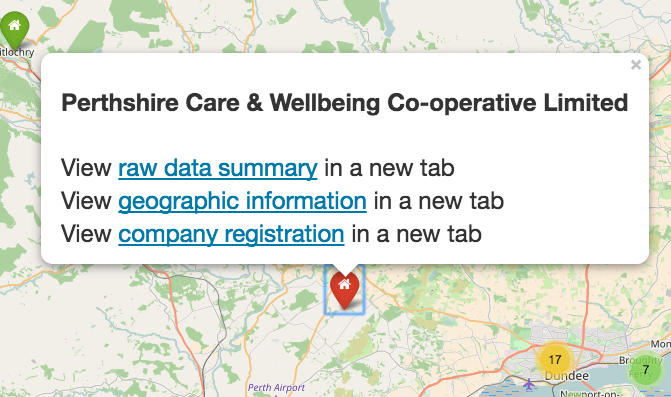
\includegraphics{map-app-popup-screenshot.png}
    \makebox[\textwidth]{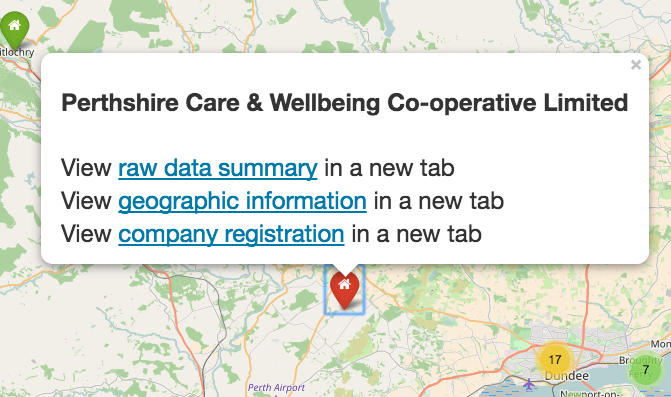
\includegraphics[width=\popupimagewidth]{map-app-popup-screenshot.png}}
    %\makebox[\textwidth]{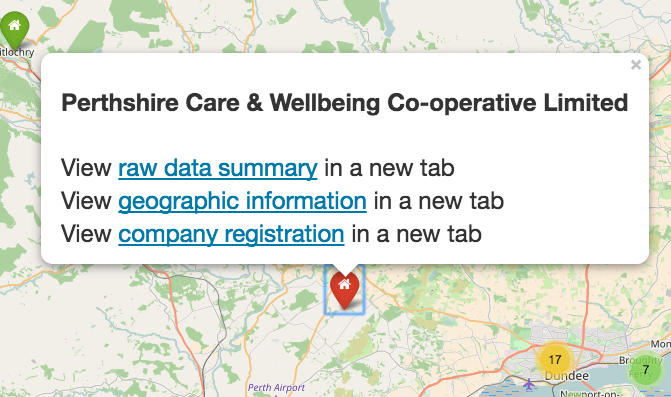
\includegraphics[width=\paperwidth]{map-app-popup-screenshot.png}}
    %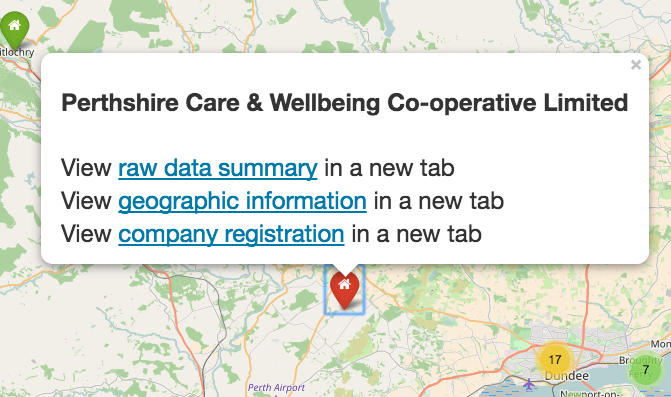
\includegraphics[height=2cm,width=2cm]{map-app-popup-screenshot.png}
  \end{center}
  \begin{itemize}
    \item
  \end{itemize}
}

\section{Conclusions}
\frame
{
  \frametitle{Lessons from re-use}
  \begin{itemize}
    \item Makes the original developers very happy
    \item Great co-operation from original developers
    \item Learn from others
    \item Answers questions you'd not know to ask \texttt{!important;}
    \item Leave things in better shape
  \end{itemize}
}
\frame
{
  \frametitle{LOD Everywhere?}
  \begin{center}
    %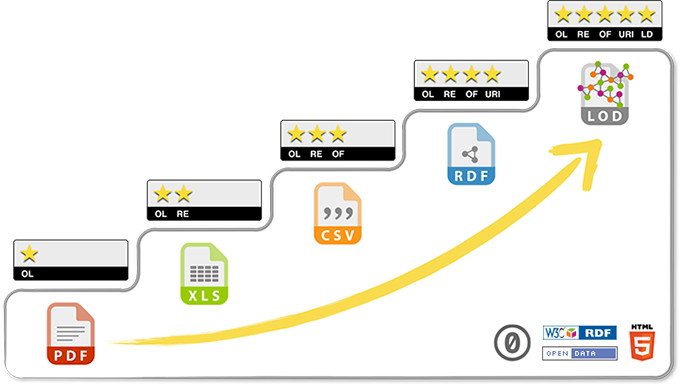
\includegraphics{5-star-steps.png}
    \makebox[\textwidth]{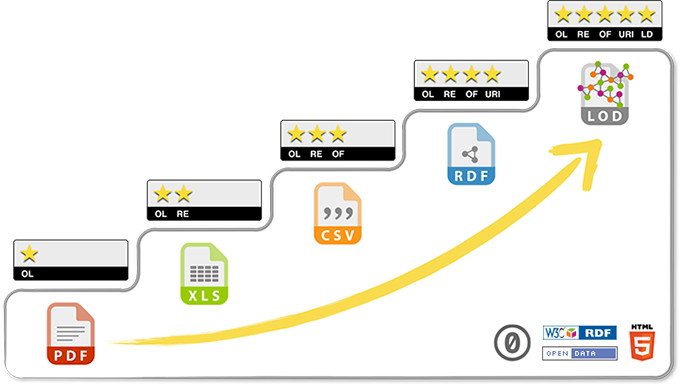
\includegraphics[width=\popupimagewidth]{5-star-steps.png}}
    %\makebox[\textwidth]{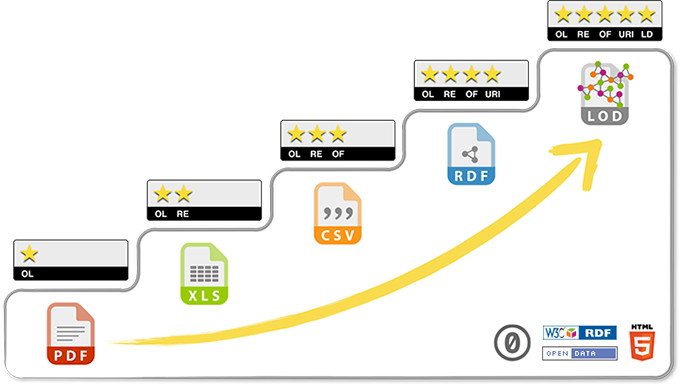
\includegraphics[width=\paperwidth]{5-star-steps.png}}
    %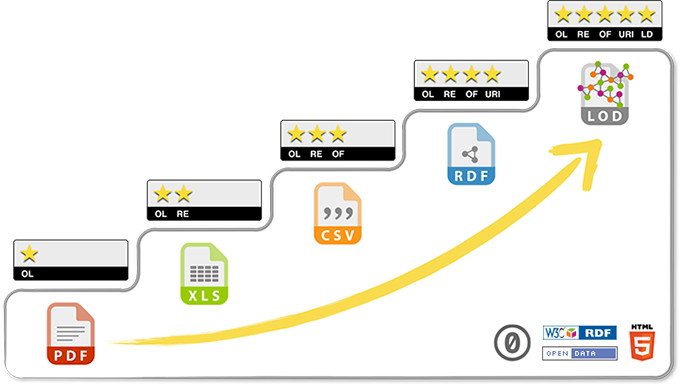
\includegraphics[height=2cm,width=2cm]{5-star-steps.png}
  \end{center}
  \begin{itemize}
    \item \url{http://5stardata.info}
  \end{itemize}
}
\frame
{
  \frametitle{The LOD approach}
  \begin{itemize}
    \item Avoid reinvention of wheels you didn't know existed
    \item Excellent for ``National Grid'' of data
    \item Easliy integrate with other data standards
    \item LOD everywhere? No!

  \end{itemize}
}
\frame
{
  \frametitle{What's next?}
  \begin{itemize}
    \item We can help
    \item How to find out more?
  \end{itemize}
}


\end{document}
